
\chapter{Homepage}

Con questo programma è possibile leggere e interrogare dispositivi compatibili 
con il protocollo Modbus sia RTU che TCP.
Avviando il programma si apre la tab principale di connessione a uno slave. Selezionare TCP
o RTU a seconda della tipologia di slave a cui ci si sta collegando. 
Per leggere slave RTU è necessario un convertitore USB-485. 
Nel caso di slave TCP a partire dalla versione v2.38
è possibile utilizzare una comunicazione criptata nella versione Modbus Secure.

\begin{figure}[H]
\centering
\includegraphics[width=0.85\textwidth]{../Img/Modbus_Client_Home_00.PNG}
\caption[Homepage]{Homepage}
\end{figure}

Per testare la connessione a un indirizzo IP utilizzare il pulsante ping,
se il ping ha successo il pulsante si colora di verde altrimenti di rosso.
Quando la connessione a uno slave va a buon fine il cubetto "Running" si colora
di verde (nel caso di connessioni RTU si considera a buon fine se riesce 
aprire correttamente la porta COM selezionata).
Nella parte seguente del documento verranno descritte le varie tab e funzioni associate.

\newpage
\section{Modbus Secure}

A partire dalla vesione 2.38 è stato introdotto il supporto
al protocollo ModBus Secure, secondo la specifica della normativa
definita nel documento MB-TCP-Security-v21\_2018-07-24.
Flaggando la spunta "Modbus Secure" si abilita la configurazione "Secure" 
come riportato nell'immagine
seguente:

\begin{figure}[H]
\centering
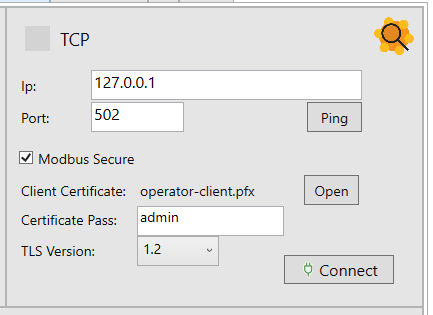
\includegraphics[width=0.6\textwidth]{../Img/ModBus_Home_Secure.PNG}
\caption[Modbus Secure]{Modbus Secure}
\end{figure}

Il protocollo Modbus Secure verrà approfondito a seguire nella
sezione \ref{secure}, a livello di configurazione lavora via TCP 
criptando la comunicazione attraverso un layer SSL/TLS.
Il protocollo Modbus Secure richiede (oltre a IP e porta)
di caricare nel client
un certificato protetto da password (da inserire nell'apposito campo).
Il certificato va caricato in formato .pfx, questo
formato contiene, assieme al certificato, anche 
la chiave privata da utilizzare per criptare la comunicazione.
Il client supporta TLS v1.2 o 1.3 (la normativa richiede v1.2 o superiore).